\begin{figure*}[!t]
    \centering
    % Row 1
    \begin{subfigure}[b]{1\textwidth}
        \centering
        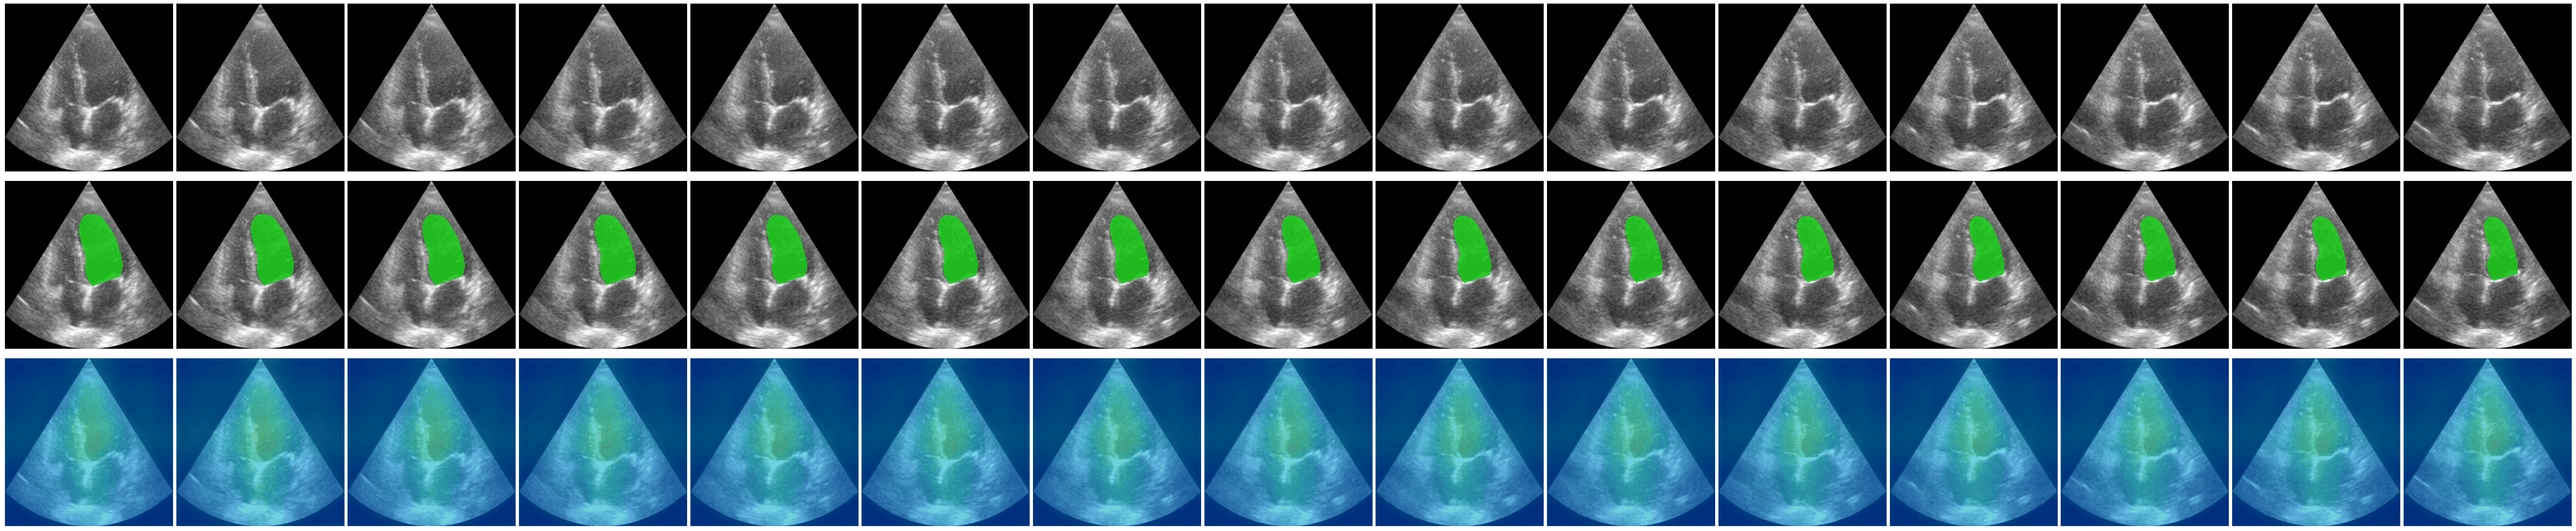
\includegraphics[width=\textwidth]{fig/train_step/It_0010_E_01_test_patient0225_4CH.pdf}
        \caption{Iteration 10, Epoch 1}
        \label{fig:training_iter10}
    \end{subfigure}
    % Row 2
    \begin{subfigure}[b]{1\textwidth}
        \centering
        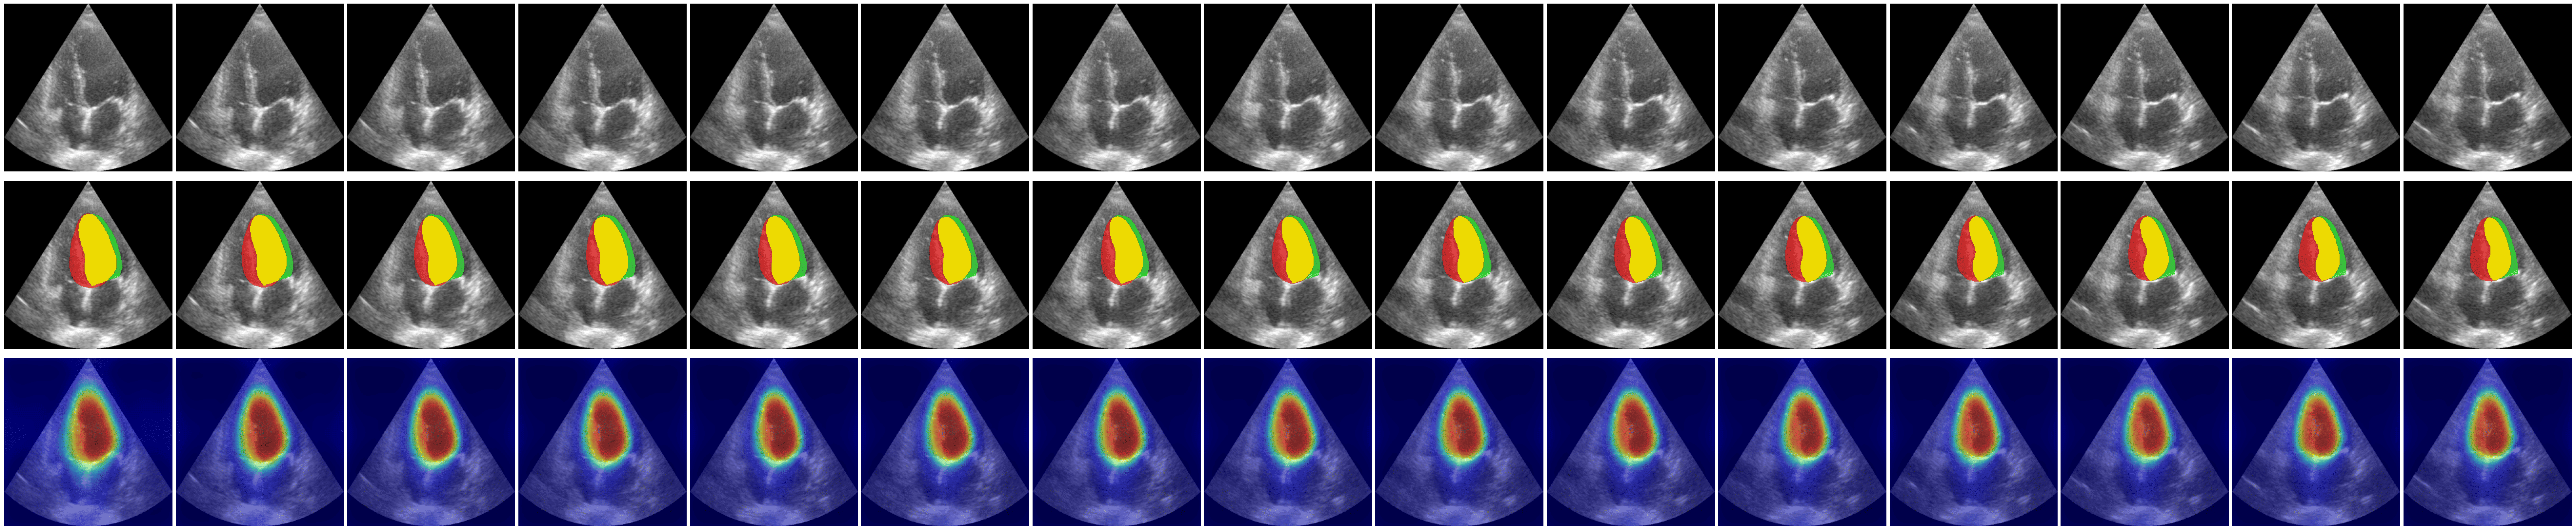
\includegraphics[width=\textwidth]{fig/train_step/It_0020_E_01_test_patient0225_4CH.pdf}
        \caption{Iteration 20, Epoch 1}
        \label{fig:training_iter20}
    \end{subfigure}
    % Row 3
    \begin{subfigure}[b]{1\textwidth}
        \centering
        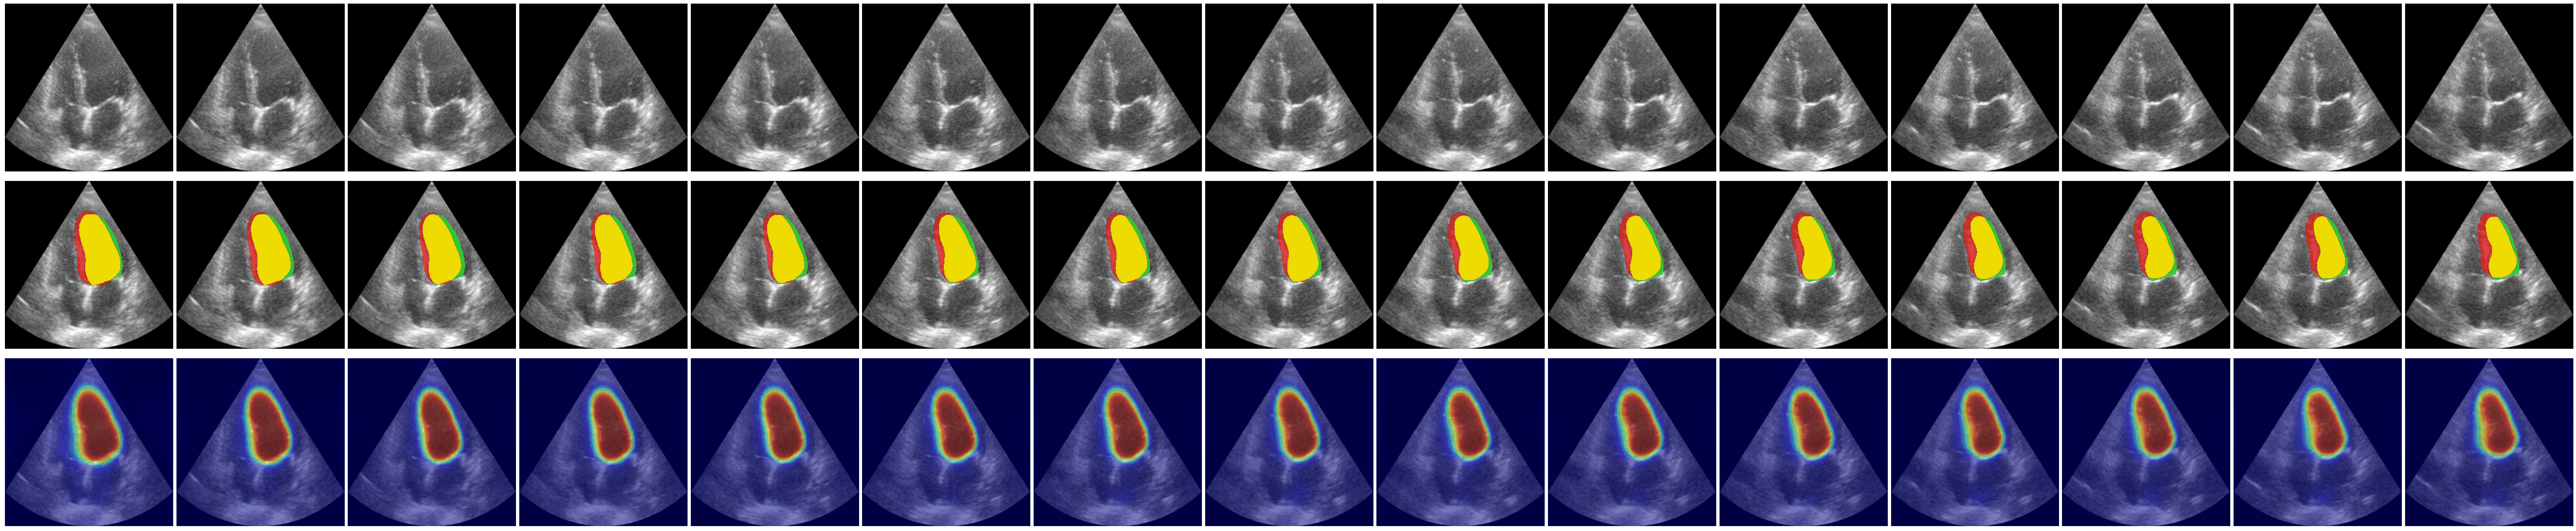
\includegraphics[width=\textwidth]{fig/train_step/It_0030_E_01_test_patient0225_4CH.pdf}
        \caption{Iteration 30, Epoch 1}
        \label{fig:training_iter30}
    \end{subfigure}
    % Row 4
    \begin{subfigure}[b]{1\textwidth}
        \centering
        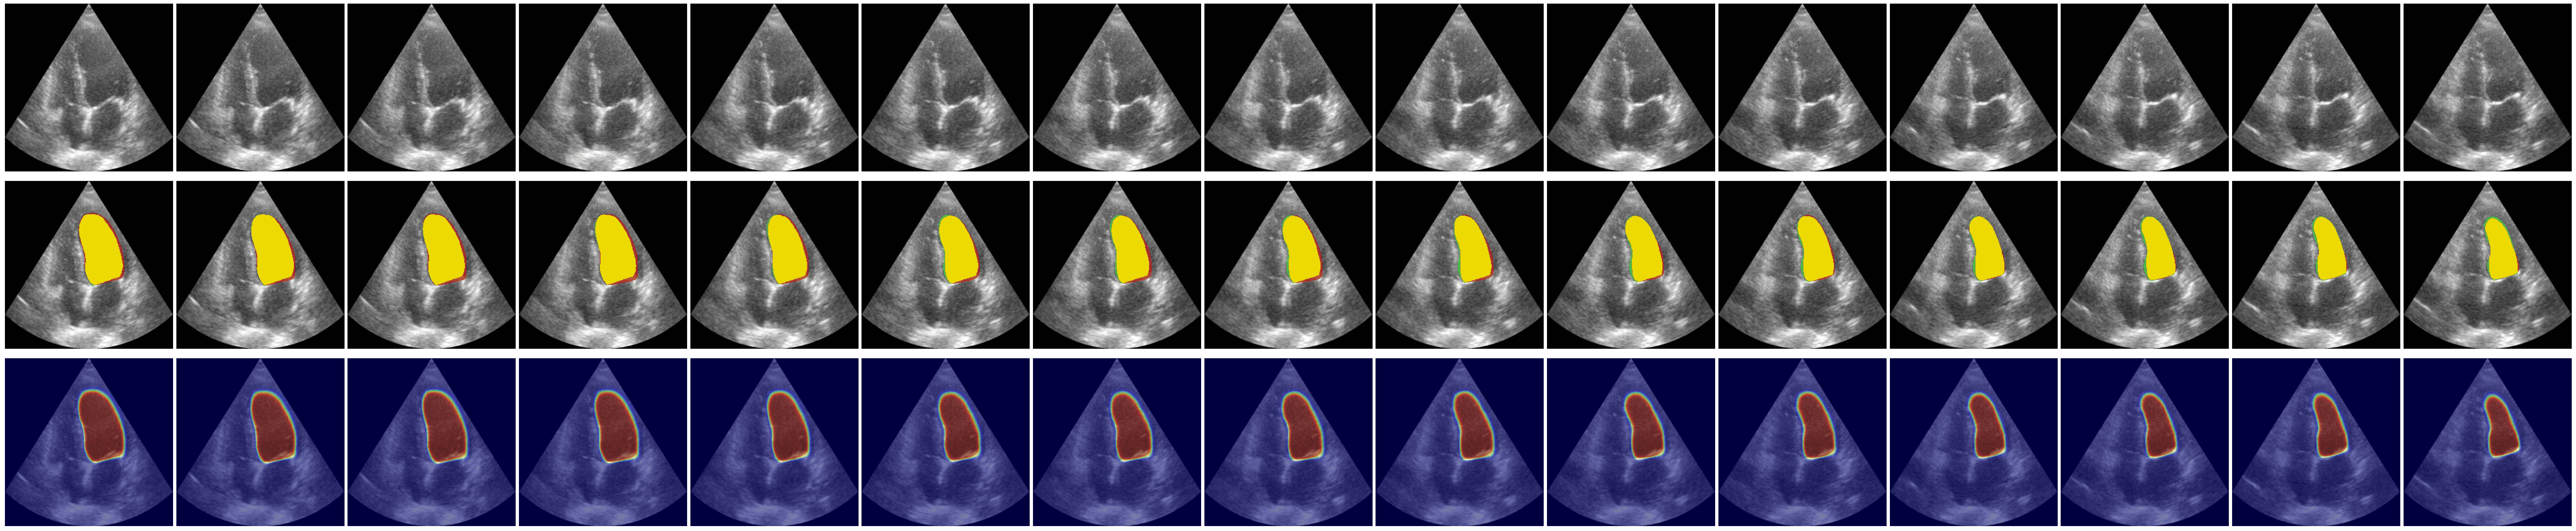
\includegraphics[width=\textwidth]{fig/train_step/It_1250_E_19_test_patient0225_4CH.pdf}
        \caption{Iteration 1250, Epoch 19}
        \label{fig:training_iter1250}
    \end{subfigure}
    %
    \caption{\textbf{Spatiotemporal training dynamics visualization.}
    Qualitative results on CAMUS patient 0225 (4-chamber view) at four training stages. For each stage (a-d), the top row displays input frames with segmentation masks, and the bottom row shows the corresponding feature activation maps. The progression from (a) to (d) illustrates the transition from diffused spatial activations and coarse masks to localized feature representations and temporally consistent segmentations throughout the cardiac cycle.}
    \label{fig:training_progression}
\end{figure*}
